\section{Experimental Studies}
\label{sec:experiment}
We examine the difference in operation of NSGAII and NOSSGA and evaluate their performance with respect to three existing methods (ASTRAL, MP-EST and STELAR) based on three simulated datasets: 10-taxon (\#estimated gene tree: 200)~\cite{bayzid2015weighted}, 11-taxon (\#estimated gene tree: 50)~\cite{chung2011comparing} and 15-taxon (\#estimated gene tree: 100)~\cite{statistical-binning}. Each of them has 10 replicates (R1 to R10). We used False Negative (FN) rate~\cite{bayzid2013naive} to measure the accuracy of the estimated species tree. FN rate expresses the fraction of edges present in the true species tree but missing in the estimated tree. %previously studied

\begin{figure}
	\begin{adjustwidth}{-4cm}{-3cm}
		\centering	
		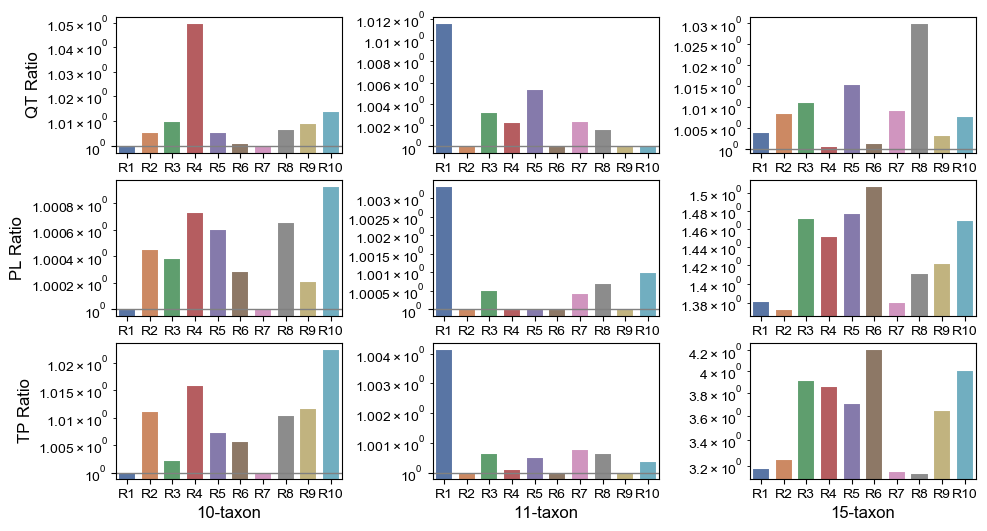
\includegraphics[width=1.6\textwidth]{Figure/tool_ratio}
		\caption{The issue of overshooting the optimization criterion beyond the true tree by existing methods. Each row shows the ratio of scores (QT/PL/TP), optimized by a particular method (ASTRAL/MP-EST/STELAR), of the true tree to that of the estimated tree by the same method.} \label{fig:tool_ratio}
	\end{adjustwidth}

\end{figure}

\subsection{Observation}
\label{subsec:observation}
At first, we present an important observation that essentially motivated us to tackle the problem of species tree estimation as a MOP. We mentioned in Section~\ref{sec:intro} that, due to limitation in available knowledge, existing methods may overshoot the criterion they try to optimize, and thus may deviate from the true tree. In Fig.~\ref{fig:tool_ratio}, we summarize our observations for three methods (ASTRAL, MP-EST and STELAR) on 10 replicates of our selected datasets. Here, the top row shows the ratio of quartet-scores (QT) of the true trees to quartet-scores (QT) of the ASTRAL-estimated trees. Likewise, the middle row shows the pseudo-likelihood (PL) ratio of the true trees and MP-EST estimated trees and the bottom row does the same with triplet (TP) ratio of STELAR. As we treat each objective as a minimization form, ideally these ratios should be 1 (marked as gray horizontal line in each plot). However, we find that in most of the cases the ratio is greater than 1. %And for 15-taxon (third column of Fig.~\ref{fig:tool_ratio}), we 


\subsection{NSGAII vs. NOSSGA}
Here we thoroughly inspect the behavioral difference between NSGAII and NOSSGA to know whether NOSSGA posses our desired properties. To ensure a level playing field, we ran both algorithms with the same configuration (independent run: 15 , population size: 100, maximum evaluations: 10000, crossover rate: 0.3, mutation rate: 1.0). For NOSSGA, we use tournament size 10.


\subsubsection{Correlation between two objectives:} We show the variation of correlation between each pair of objectives with generations for NSGAII and NOSSGA on three datasets in Fig.~\ref{fig:gen_wise_correlation}. The plotted correlation coefficients are averaged over 15 runs and 10 replicates. We see that, contrary to NSGAII, NOSSGA is able to avoid conflict between any two objectives along the whole period according to our expectation\footnote{Nayeem link it to the method section in algo}. 

\begin{figure}[!htbp]
	%\scriptsize
	\centering
	\begin{adjustwidth}{-1cm}{-1cm}
		\begin{subfigure}[b]{0.4\textwidth}
			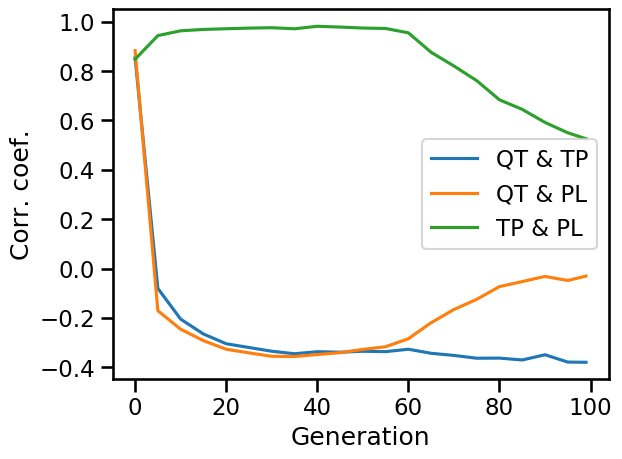
\includegraphics[width=\textwidth]{Figure/10-taxon_NSGAII_corr_plot}
			\caption{NSGAII: 10-taxon}
			%\label{fig:con_pr06}
		\end{subfigure}%
		\begin{subfigure}[b]{0.4\textwidth}
			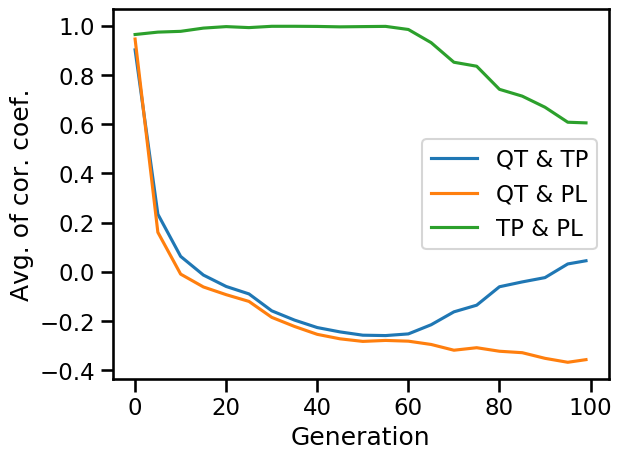
\includegraphics[width=\textwidth]{Figure/11-taxon_NSGAII_corr_plot}
			\caption{NSGAII: 11-taxon}
			%\label{fig:con_pr07}
		\end{subfigure}%
		\begin{subfigure}[b]{0.4\textwidth}
			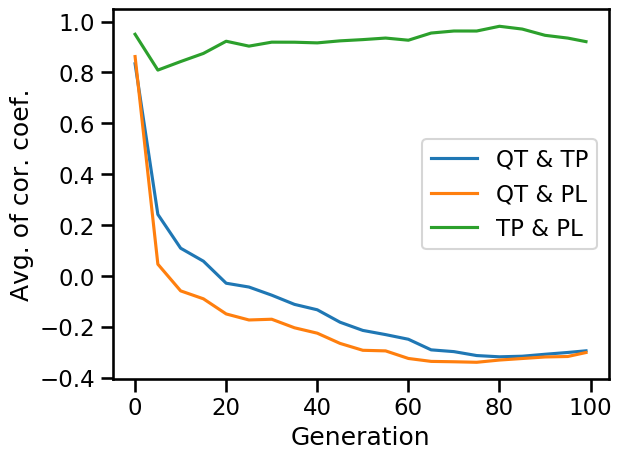
\includegraphics[width=\textwidth]{Figure/15-taxon_NSGAII_corr_plot}
			\caption{NSGAII: 15-taxon}
			%\label{fig:con_pr09}
		\end{subfigure}	
		\begin{subfigure}[b]{0.4\textwidth}
			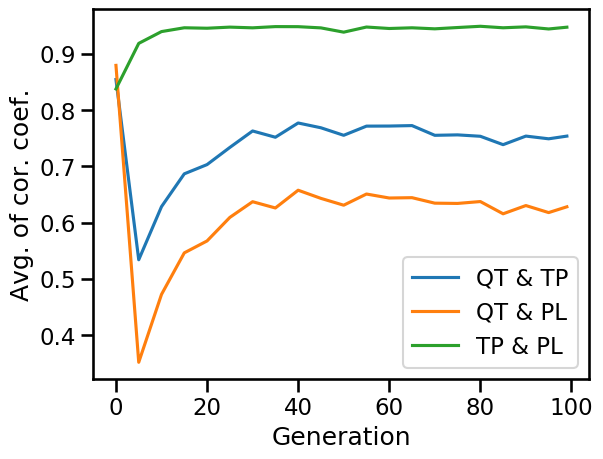
\includegraphics[width=\textwidth]{Figure/10-taxon_NOSSGA_corr_plot}
			\caption{NOSSGA: 10-taxon}
			%\label{fig:con_pr06}
		\end{subfigure}%
		\begin{subfigure}[b]{0.4\textwidth}
			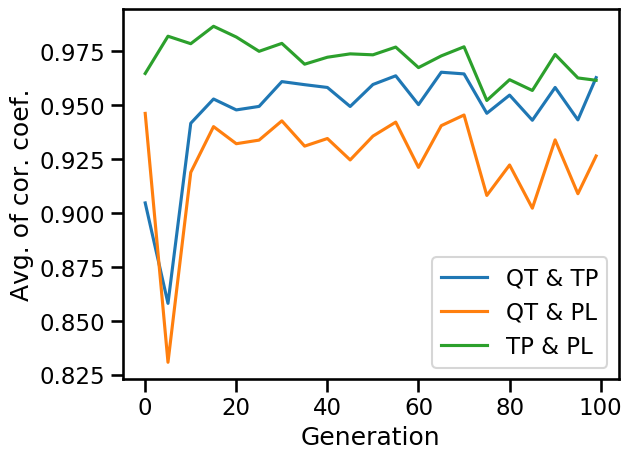
\includegraphics[width=\textwidth]{Figure/11-taxon_NOSSGA_corr_plot}
			\caption{NOSSGA: 11-taxon}
			%\label{fig:con_pr07}
		\end{subfigure}%
		\begin{subfigure}[b]{0.4\textwidth}
			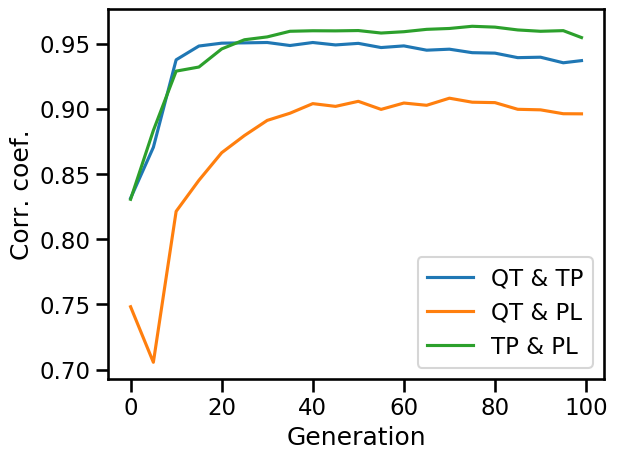
\includegraphics[width=\textwidth]{Figure/15-taxon_NOSSGA_corr_plot}
			\caption{NOSSGA: 15-taxon}
			%\label{fig:con_pr09}
		\end{subfigure}
		\caption{Variation of correlation between each pair of objectives with generations for NSGAII and NOSSGA on three datasets. 
			%The plotted correlation coefficients are averaged over 15 runs and 10 replicates. 
			%In each plot (algorithm: dataset), the correlation coefficient of each point are averaged over 15 runs and 10 replicates.
		}
		\label{fig:gen_wise_correlation}
	\end{adjustwidth}
\end{figure}

\subsubsection{Diversity of objectives and FN rate:}\label{subsubsec:diversity} Fig.~\ref{fig:gen_wise_std_dev} shows the variation of standard deviation of three objectives and FN rates\footnote{The knowledge of FN rate is absent to the EMOs.} in the population with generations for NSGAII and NOSSGA on three datasets. In each plot, the standard deviation values are averaged over 15 runs and 10 replicates. This figures establish that NSGAII loses diversity at early stages possibly due to discarding dominated solutions.    
\begin{figure}[!htbp]
	\centering
	\begin{adjustwidth}{-1cm}{-1cm}
		\begin{subfigure}[b]{0.4\textwidth}
			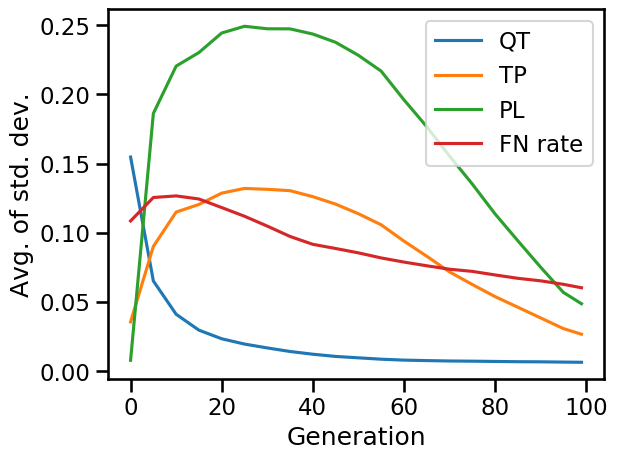
\includegraphics[width=\textwidth]{Figure/10-taxon_NSGAII_std_dev}
			\caption{NSGAII: 10-taxon}
			%\label{fig:con_pr06}
		\end{subfigure}%
		\begin{subfigure}[b]{0.4\textwidth}
			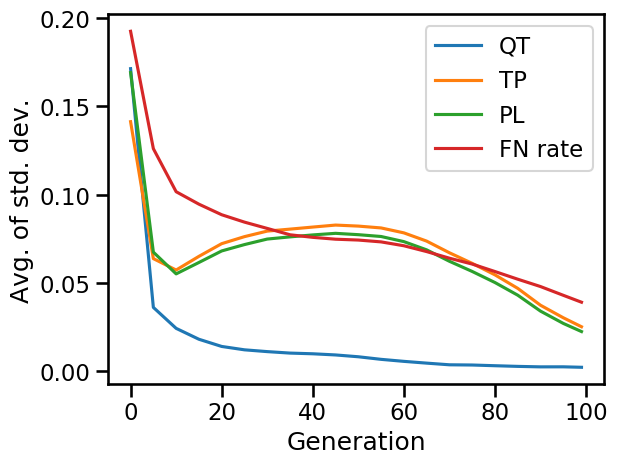
\includegraphics[width=\textwidth]{Figure/11-taxon_NSGAII_std_dev}
			\caption{NSGAII: 11-taxon}
			%\label{fig:con_pr07}
		\end{subfigure}%
		\begin{subfigure}[b]{0.4\textwidth}
			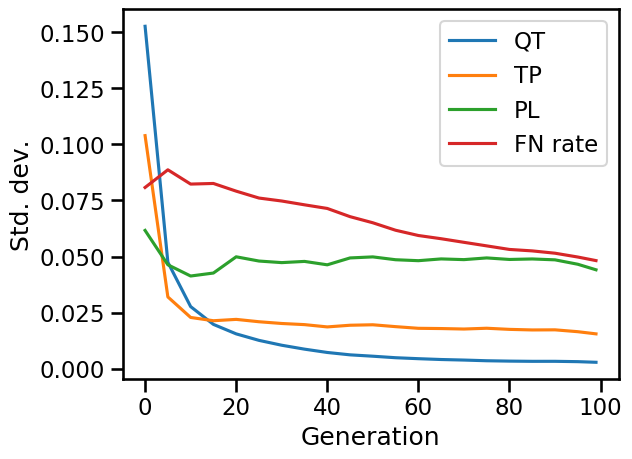
\includegraphics[width=\textwidth]{Figure/15-taxon_NSGAII_std_dev}
			\caption{NSGAII: 15-taxon}
			%\label{fig:con_pr09}
		\end{subfigure}
		\begin{subfigure}[b]{0.4\textwidth}
			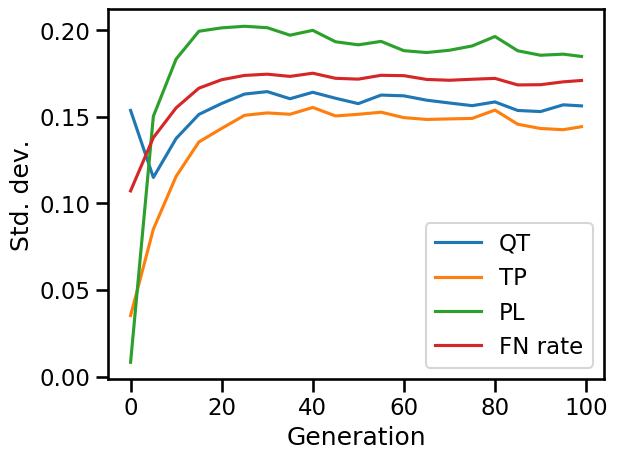
\includegraphics[width=\textwidth]{Figure/10-taxon_NOSSGA_std_dev}
			\caption{NOSSGA: 10-taxon}
			%\label{fig:con_pr06}
		\end{subfigure}%
		\begin{subfigure}[b]{0.4\textwidth}
			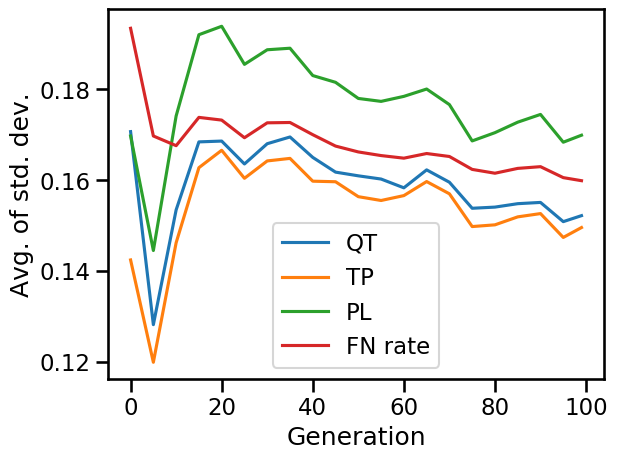
\includegraphics[width=\textwidth]{Figure/11-taxon_NOSSGA_std_dev}
			\caption{NOSSGA: 11-taxon}
			%\label{fig:con_pr07}
		\end{subfigure}%
		\begin{subfigure}[b]{0.4\textwidth}
			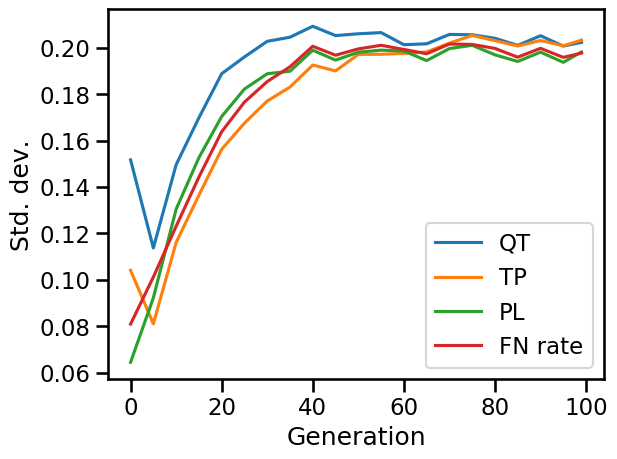
\includegraphics[width=\textwidth]{Figure/15-taxon_NOSSGA_std_dev}
			\caption{NOSSGA: 15-taxon}
			%\label{fig:con_pr09}
		\end{subfigure}
		\caption{Variation of standard deviation of three objectives and FN rates in the population with generations for NSGAII and NOSSGA on three datasets.
			% on three datasets. The plotted standard deviations are averaged over 15 runs and 10 replicates. 
		}
		\label{fig:gen_wise_std_dev}
	\end{adjustwidth}
\end{figure}

\subsubsection{Improvement in objectives and FN rate:} Now we observe how the best (minimum) value of three objectives\footnote{we treated each objective as a minimization} and FN rate\footnote{lower is better} in the population improves across generations for NSGAII and NOSSGA as depicted in Fig.~\ref{fig:gen_wise_min}. The plotted minimum values are averaged over 15 runs and 10 replicates. NSGAII allows the objectives (except PL\footnote{To decrease the large runtime of PL calculation using MP-EST, we decreased the default iteration count}) to improve as much as possible which causes the resultant species tree to deviate from the true tree. As a result, the best FN rate of NSGAII starts to degrade after a particular generation. On the other hand, to avoid such deviation, NOSGGA restrict the objectives to improve after a certain point in time. So its FN rate continues to improve.
\begin{figure}[!htbp]
	\centering
	\begin{adjustwidth}{-1cm}{-1cm}
		\begin{subfigure}[b]{0.4\textwidth}
			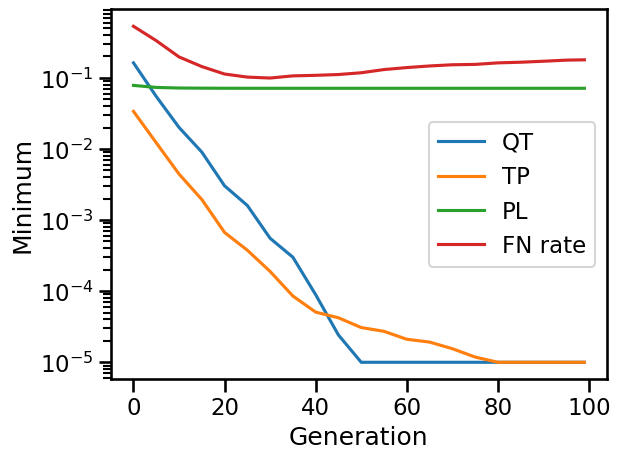
\includegraphics[width=\textwidth]{Figure/10-taxon_NSGAII_minimum}
			\caption{NSGAII: 10-taxon}
			%\label{fig:con_pr06}
		\end{subfigure}%
		\begin{subfigure}[b]{0.4\textwidth}
			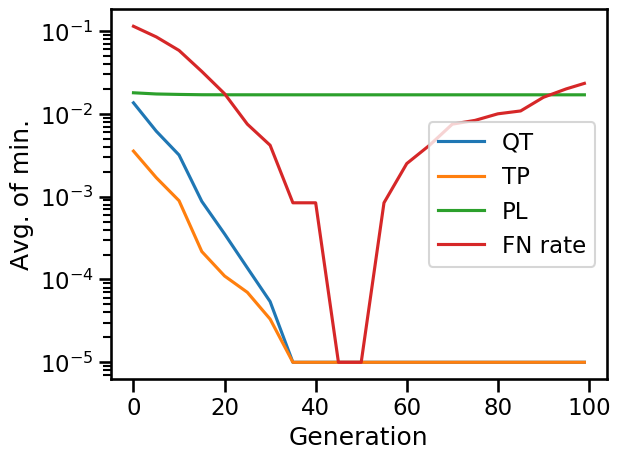
\includegraphics[width=\textwidth]{Figure/11-taxon_NSGAII_minimum}
			\caption{NSGAII: 11-taxon}
			%\label{fig:con_pr07}
		\end{subfigure}%
		\begin{subfigure}[b]{0.4\textwidth}
			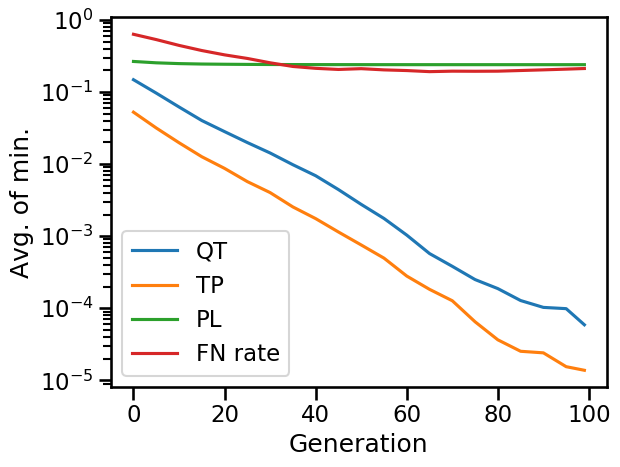
\includegraphics[width=\textwidth]{Figure/15-taxon_NSGAII_minimum}
			\caption{NSGAII: 15-taxon}
			%\label{fig:con_pr09}
		\end{subfigure}
		\begin{subfigure}[b]{0.4\textwidth}
			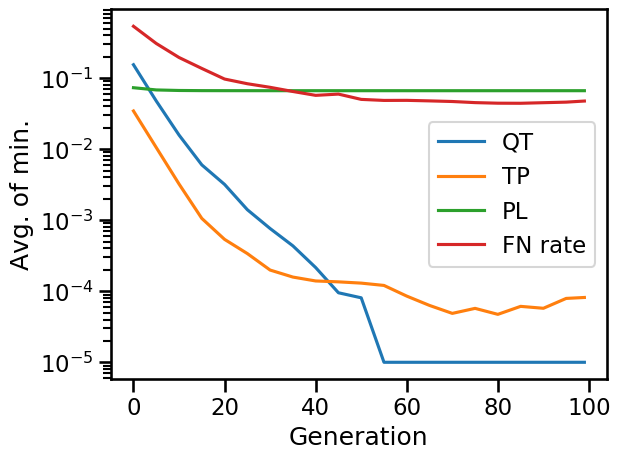
\includegraphics[width=\textwidth]{Figure/10-taxon_NOSSGA_minimum}
			\caption{NOSSGA: 10-taxon}
			%\label{fig:con_pr06}
		\end{subfigure}%
		\begin{subfigure}[b]{0.4\textwidth}
			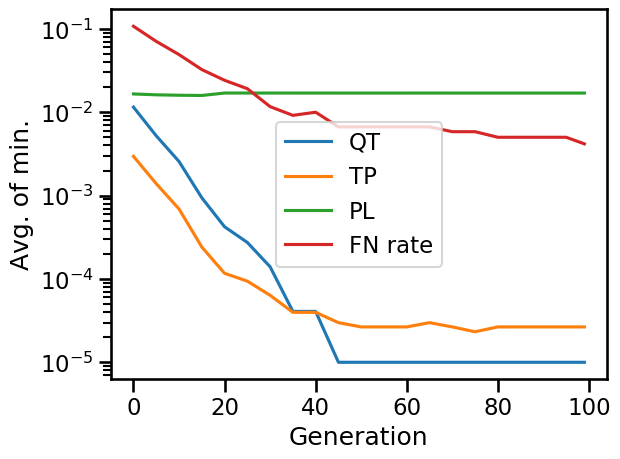
\includegraphics[width=\textwidth]{Figure/11-taxon_NOSSGA_minimum}
			\caption{NOSSGA: 11-taxon}
			%\label{fig:con_pr07}
		\end{subfigure}%
		\begin{subfigure}[b]{0.4\textwidth}
			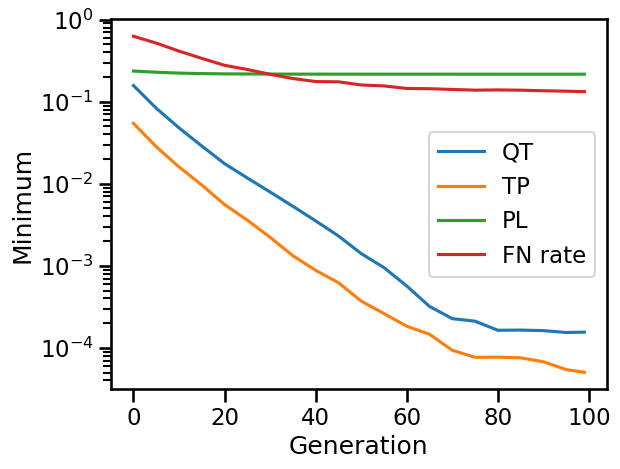
\includegraphics[width=\textwidth]{Figure/15-taxon_NOSSGA_minimum}
			\caption{NOSSGA: 15-taxon}
			%\label{fig:con_pr09}
		\end{subfigure}
		\caption{Variation of minimum of three objectives and FN rates in the population with generations for NSGAII and NOSSGA on three datasets.
			%The plotted minimum values are averaged over 15 runs and 10 replicates. 
		}
		\label{fig:gen_wise_min}
	\end{adjustwidth}
\end{figure}

\subsubsection{Comparison based on hypervolume:} We mentioned earlier that for the problem that we deal in this paper is different than the traditional MOPs. Importantly, the definition of convergence for MOPs is not applicable for our problem. To explore this issue, we compare NSGAII and NOSSGA in terms of hypervolume (HV)~\cite{zitzler1999multiobjective} which is probably the most popular measure to evaluate the performance of an EMO. HV captures both convergence and diversity in a single real-value. For MOPs with all minimization objectives, a higher value of HV is desirable. In Fig.~\ref{fig:gen_wise_hv}, we plot the HV values averaged over 15 runs and 10 replicates. From these results, it is difficult to differentiate between these two algorithms. Both of their HV values get saturated at early generation. Interestingly, according to HV, NOSSGA seems better than NSGAII. This is probably due to the loss of diversity at an early stage as we saw earlier. 
\begin{figure}[!htbp]
	\centering
	\begin{adjustwidth}{-1cm}{-1cm}
		\begin{subfigure}[b]{0.4\textwidth}
			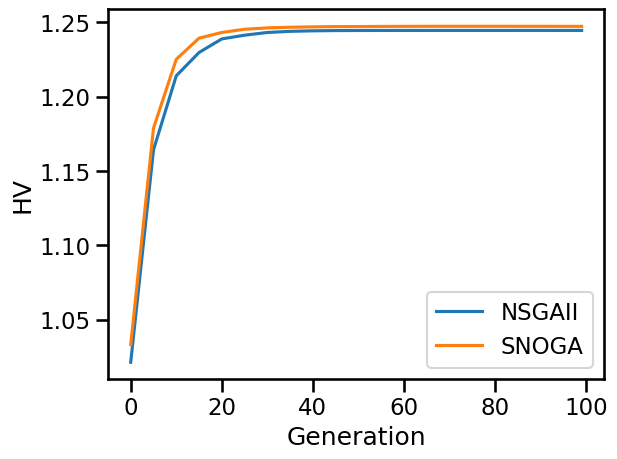
\includegraphics[width=\textwidth]{Figure/10-taxon_hv}
			\caption{10-taxon}
			%\label{fig:con_pr06}
		\end{subfigure}%
		\begin{subfigure}[b]{0.4\textwidth}
			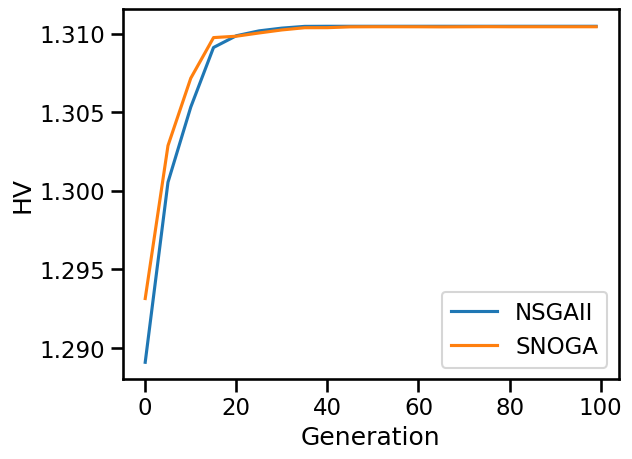
\includegraphics[width=\textwidth]{Figure/11-taxon_hv}
			\caption{11-taxon}
			%\label{fig:con_pr07}
		\end{subfigure}%
		\begin{subfigure}[b]{0.4\textwidth}
			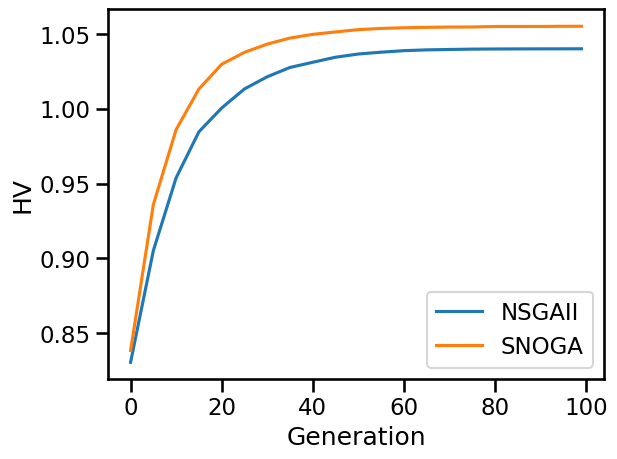
\includegraphics[width=\textwidth]{Figure/15-taxon_hv}
			\caption{15-taxon}
			%\label{fig:con_pr09}
		\end{subfigure}
		\caption{Variation of HV with generations for NSGAII and NOSSGA on three datasets.}
		\label{fig:gen_wise_hv}
	\end{adjustwidth}
\end{figure}
\subsubsection{Tree accuracy:} Finally we compare NSGAII and NOSGGA in terms of the tree accuracy for 10 replicates of each dataset. So we graphically summarize the FN rate (a lower value means more accurate) of the best trees from the final population of 15 independent runs using boxplots in Fig.~\ref{fig:emo_compare}. We observe that, NOSSGA can offer much better solutions than NSGAII in almost all cases. In some cases, the two algorithm perform equally.
\begin{figure}
	\centering
	\begin{adjustwidth}{-2cm}{-2cm}
		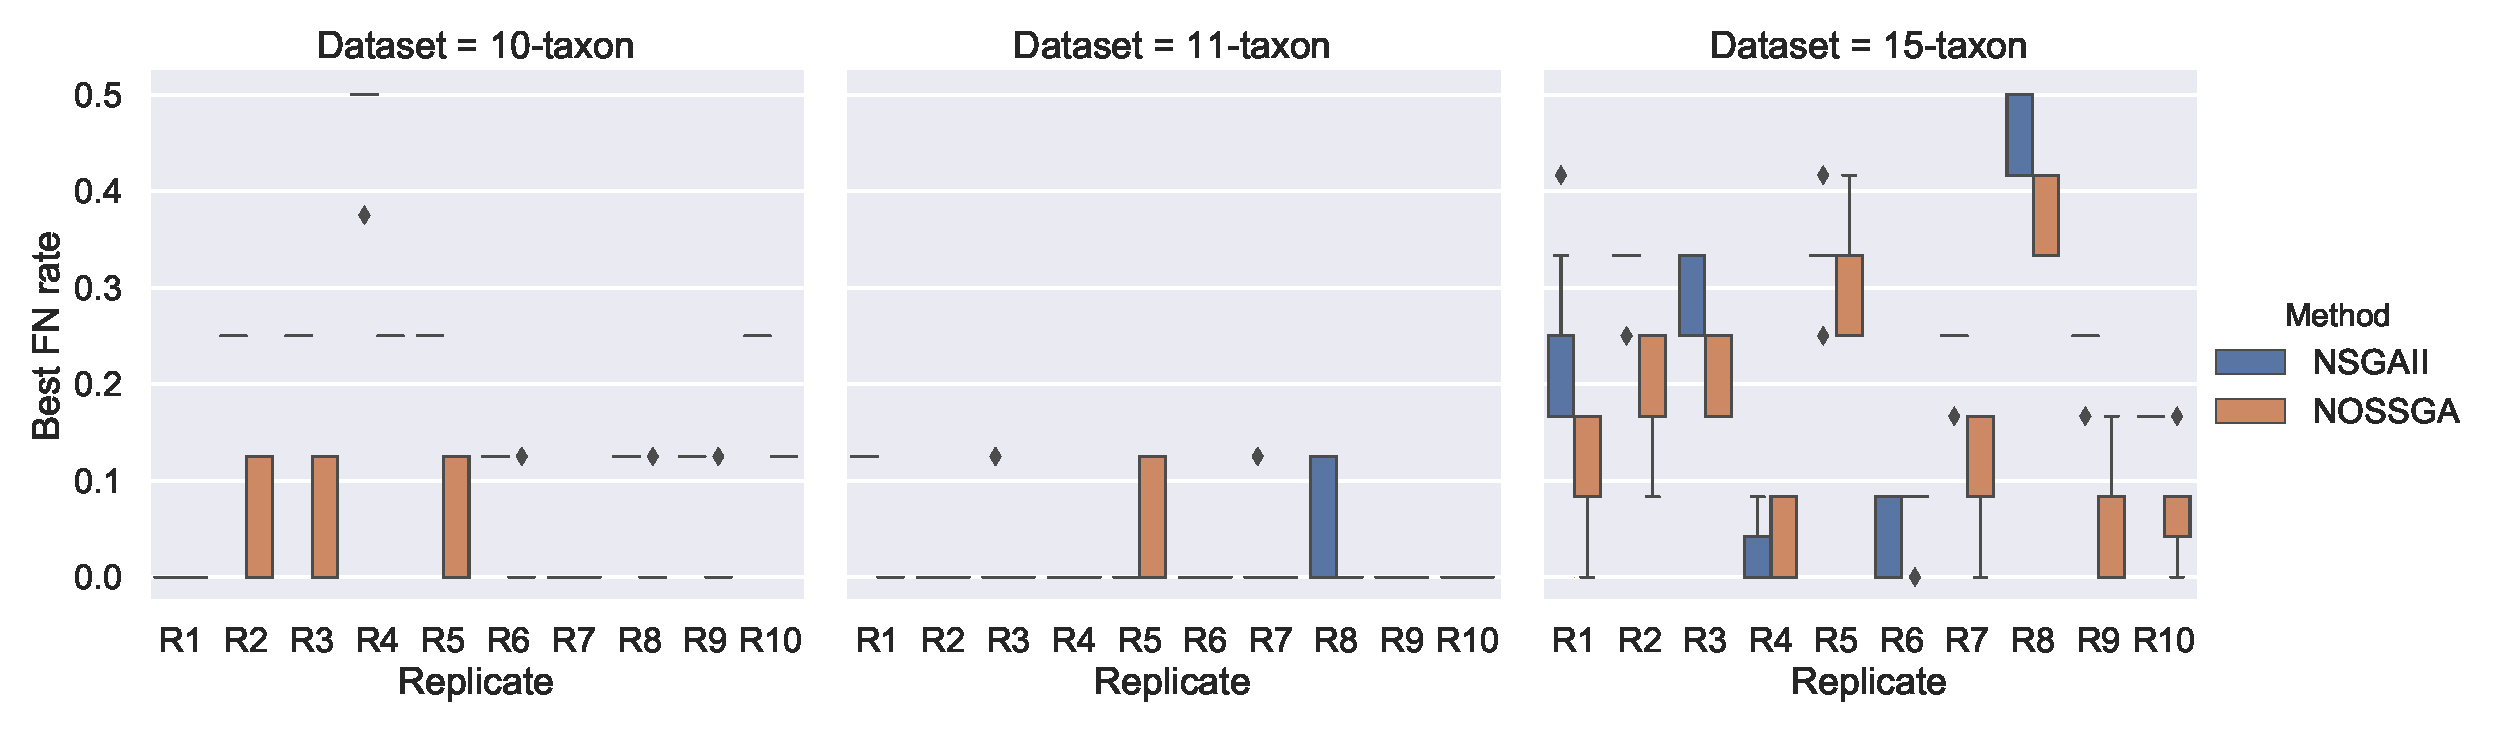
\includegraphics[width=1.5\textwidth]{Figure/emo_boxplot}
		\caption{Accuracy of the best estimated species trees extracted from the final population of NSGAII and NOSSGA on each dataset having 10 replicate.} \label{fig:emo_compare}
	\end{adjustwidth}
\end{figure}

\begin{figure}
	\begin{adjustwidth}{0cm}{0cm}
		\centering
		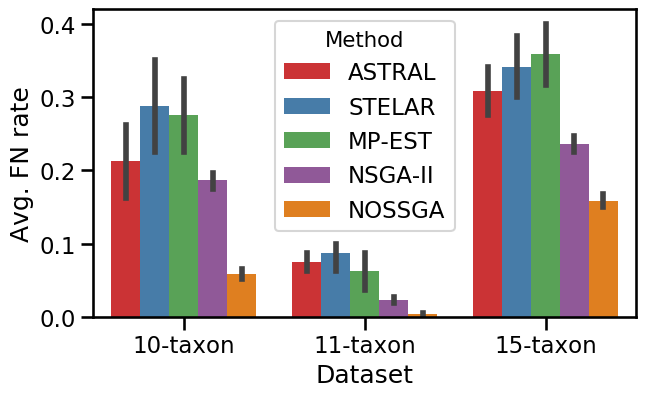
\includegraphics[width=0.8\textwidth]{Figure/all_dataset_compare}
		\caption{Performance comparison of ASTRAL, STELAR, MP-EST, NSGAII and NOSSGA on three datasets. 
			%We show the average FN rates with standard error bars over 10 replicates
		} \label{fig:compare_exisitng_methods}
	\end{adjustwidth}
\end{figure}

\subsection{Comparison with Existing Methods}
We evaluated the best trees offered by NSGAII and NOSSGA in comparison with the output of ASTRAL, MP-EST and STELAR. ASTRAL and MP-EST are two of the most widely used and accurate
summary methods. We ran the exact version of ASTRAL and STELAR, which are guaranteed to return the globally optimal tree. And for MP-EST, we ran with 10 random starting points and selected the species tree with the
highest PL value. For each dataset, we show the average FN rates with standard error bars over 10 replicates in Fig.~\ref{fig:compare_exisitng_methods}. We find that NOSSGA offers the most accuracy. In all datasets, the accuracy of NOSSGA is at least 2X than ASTRAL. Even the basic NSGAII is more accurate than all of the three existing methods. These results clearly demonstrate the benefit of treating this problem as a MOP. 


%\subsection{Discussion}

\begin{comment}
\begin{figure}[!htbp]
	\centering
	\begin{adjustwidth}{-1cm}{}
	\begin{subfigure}[b]{0.55\textwidth}
		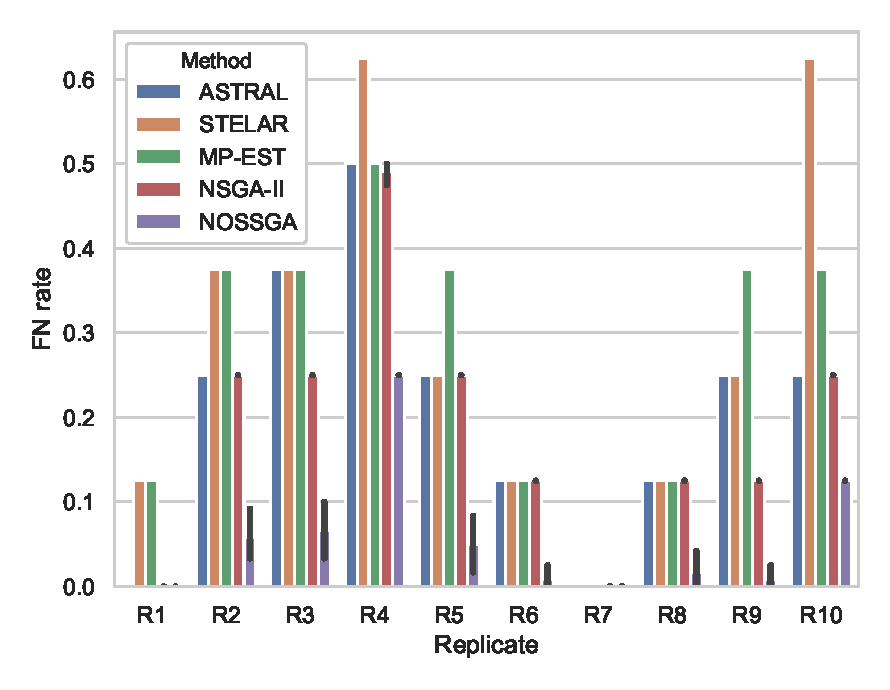
\includegraphics[width=\textwidth]{Figure/10-taxon_10_replicates}
		\caption{10-taxon}
		%\label{fig:con_pr06}
	\end{subfigure}%
	\begin{subfigure}[b]{0.55\textwidth}
		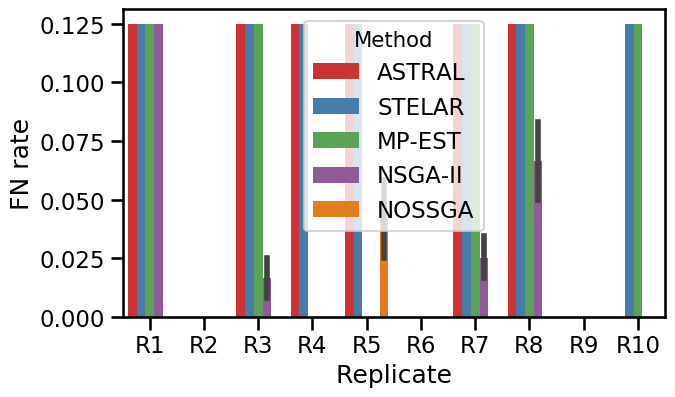
\includegraphics[width=\textwidth]{Figure/11-taxon_10_replicates}
		\caption{11-taxon}
		%\label{fig:con_pr07}
	\end{subfigure}%
%	\newline

	\begin{subfigure}[b]{0.55\textwidth}
		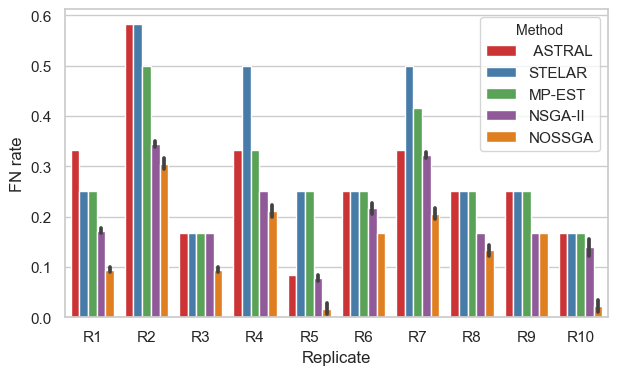
\includegraphics[width=\textwidth]{Figure/15-taxon_10_replicates}
		\caption{15-taxon}
		%\label{fig:con_pr09}
	\end{subfigure}
	\begin{subfigure}[b]{0.55\textwidth}
		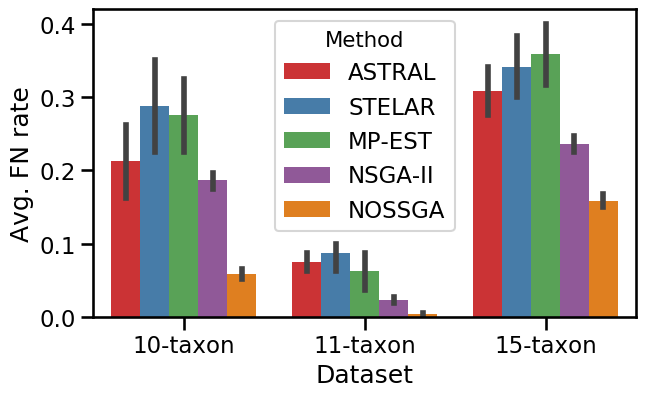
\includegraphics[width=\textwidth]{Figure/all_dataset_compare}
		\caption{Summary}
		%\label{fig:con_pr09}
	\end{subfigure}%

	\caption{Comparison of ASTRAL, STELAR, MP-EST, NSGAII and NOSSGA on 10 replicates of 3 datasets.}
	\label{fig:datasets}
\end{adjustwidth}
\end{figure}



\begin{figure}[!htbp]
\centering
\begin{adjustwidth}{-1cm}{}
\begin{subfigure}[b]{0.48\textwidth}
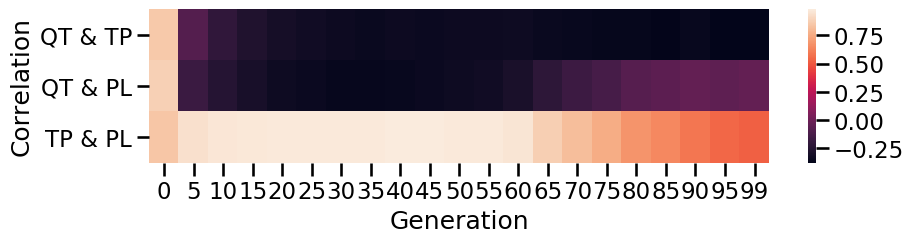
\includegraphics[width=\textwidth]{Figure/10-taxon_NSGA-II_heatmap}
\caption{NSGAII: 10-taxon}
%\label{fig:con_pr06}
\end{subfigure}%
\begin{subfigure}[b]{0.4\textwidth}
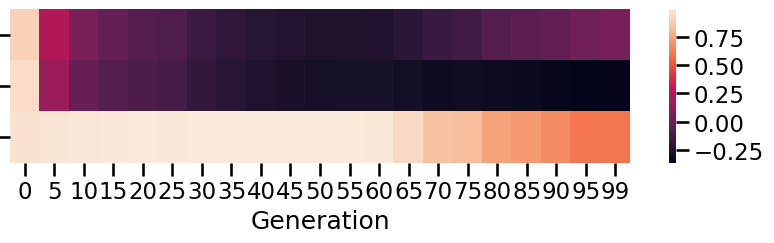
\includegraphics[width=\textwidth]{Figure/11-taxon_NSGA-II_heatmap}
\caption{NSGAII: 11-taxon}
%\label{fig:con_pr07}
\end{subfigure}%
\begin{subfigure}[b]{0.4\textwidth}
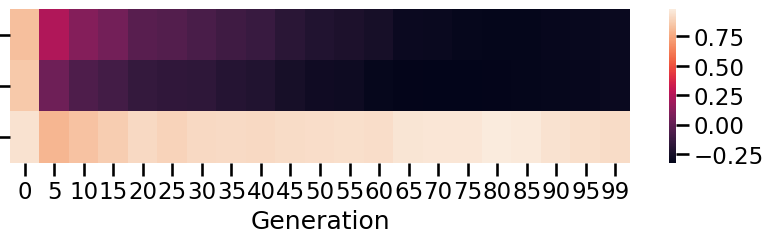
\includegraphics[width=\textwidth]{Figure/15-taxon_NSGA-II_heatmap}
\caption{NSGAII: 15-taxon}
%\label{fig:con_pr09}
\end{subfigure}

\begin{subfigure}[b]{0.48\textwidth}
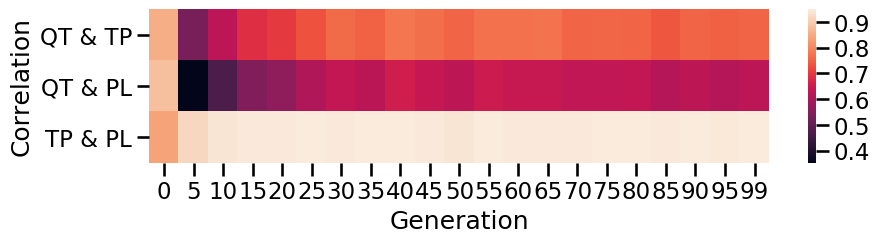
\includegraphics[width=\textwidth]{Figure/10-taxon_NOSSGA_heatmap}
\caption{NOSSGA: 10-taxon}
%\label{fig:con_pr06}
\end{subfigure}%
\begin{subfigure}[b]{0.4\textwidth}
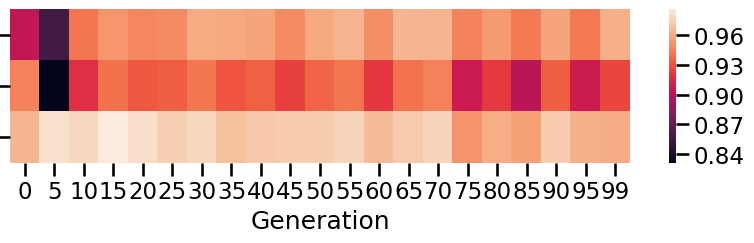
\includegraphics[width=\textwidth]{Figure/11-taxon_NOSSGA_heatmap}
\caption{NOSSGA: 11-taxon}
%\label{fig:con_pr07}
\end{subfigure}%
\begin{subfigure}[b]{0.4\textwidth}
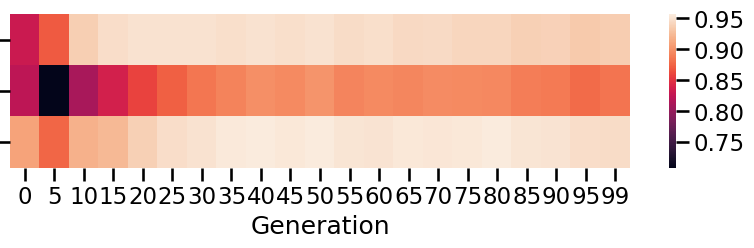
\includegraphics[width=\textwidth]{Figure/15-taxon_NOSSGA_heatmap}
\caption{NOSSGA: 15-taxon}
%\label{fig:con_pr09}
\end{subfigure}
\caption{Correlation between each pair of objectives as the generation of an EMO progresses. For each dataset, we average the correlation coefficient over 15 runs and 10 replicates.}
\label{fig:gen_wise_correlation}
\end{adjustwidth}
\end{figure}
%\begin{figure}
%	\centering
%	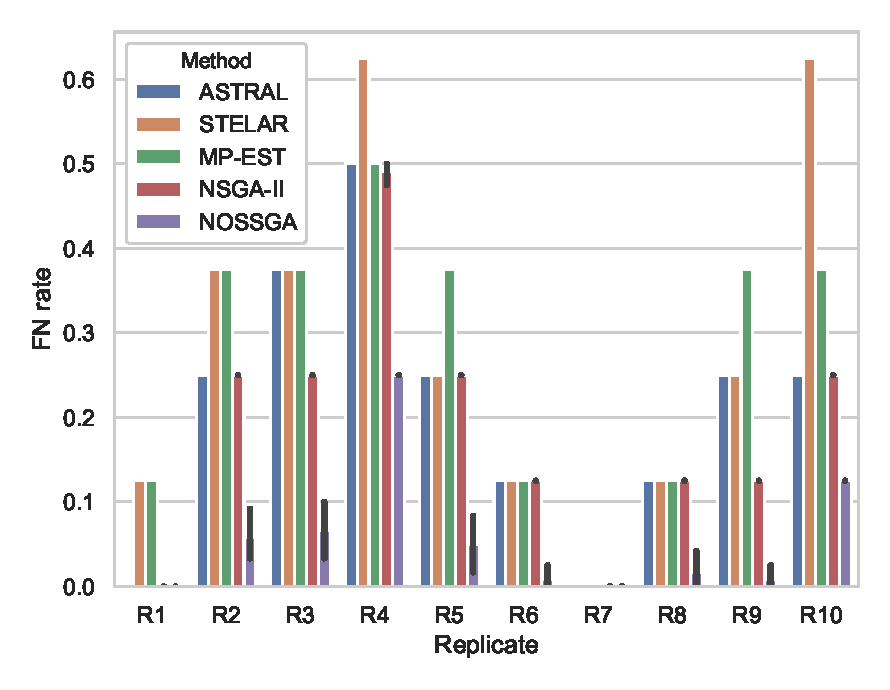
\includegraphics[width=0.6\textwidth]{Figure/10-taxon_10_replicates}
%	\caption{10-taxon.} \label{fig1}
%\end{figure}
%\begin{figure}
%	\centering
%	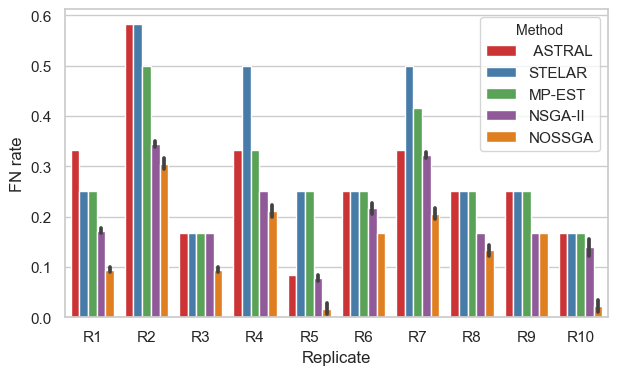
\includegraphics[width=0.6\textwidth]{Figure/15-taxon_10_replicates}
%	\caption{15-taxon.} \label{fig2}
%\end{figure}
\subsection{Results on 10-taxon dataset}
\subsection{Results on 11-taxon dataset}
\subsection{Results on 15-taxon dataset}
\end{comment}

